\chapter{Microsoft HoloLens 2}
Il primo sistema operativo olografico al mondo è stato introdotto da Microsoft nel 2015 appositamente per dispositivi HoloLens.
Originariamente noto come \textit{Windows Holographic}, questa variante del sistema operativo Windows ha fornito una piattaforma di realtà mista che potesse essere sperimentata dagli sviluppatori e ha permesso di integrare le app universali di Windows esistenti in questo nuovo ambiente.
Successivamente, Microsoft ha consentito ai visori compatibili di utilizzare un ambiente \textit{Windows Mixed Reality} all'interno di Windows stesso, integrando parte dell'esperienza utente introdotta in precedenza da Microsoft HoloLens.

\section{Specifiche Tecniche del Device}\label{sec:Sezione2.1}

Come detto in precedenza, HoloLens 2 è un visore per la realtà mista annunciato da Microsoft nel Mobile World Congress del 2019.
Questa nuova versione va a rimpiazzare la prima generazione di HoloLens, introdotta nel 2016.
Di seguito vengono presentate le caratteristiche hardware del dispositivo (Figura \ref{fig:figure2}), comparate anche a quelle del suo predecessore.

\begin{figure}[t]
    \centering
    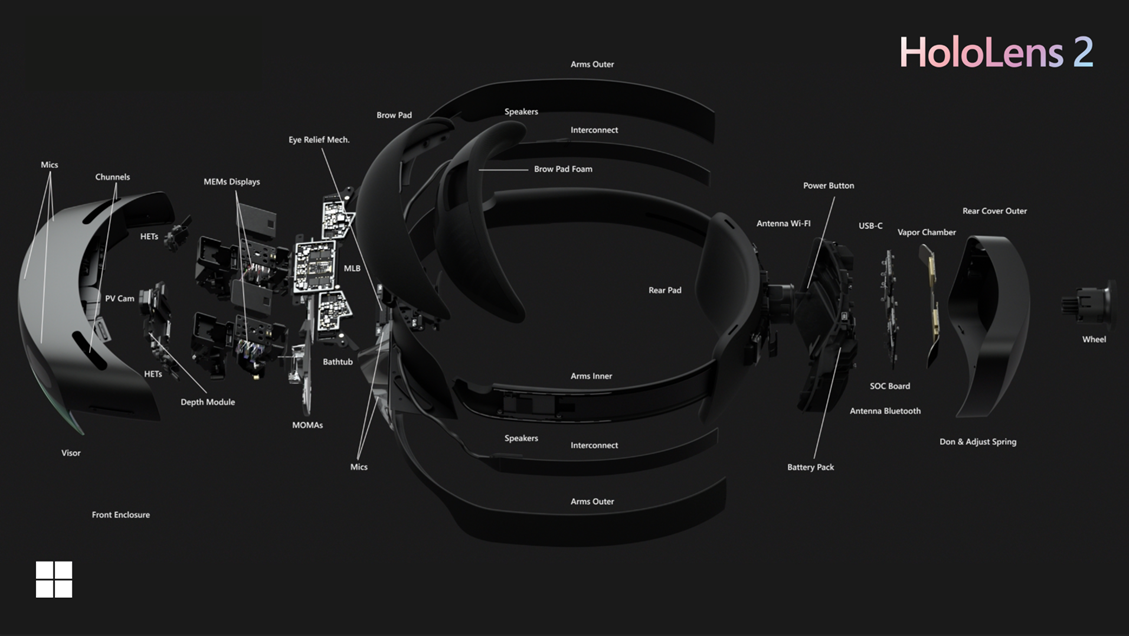
\includegraphics[width=\textwidth]{images/hololens2-breakdown.png}
    \caption{Componenti di HoloLens 2.}
    \label{fig:figure2}
\end{figure}

HoloLens 2 vanta un campo visivo ampliato e una risoluzione ottica notevolmente aumentata, passando da circa 720p a 2K di risoluzione per occhio. Ciò consente agli utenti di visualizzare ologrammi molto più dettagliati e di vederli da angoli più ampi, piuttosto che dover rimanere concentrati su punti molto specifici.

\begin{center}
    \begin{tabular}{ p{6cm} p{7cm} }
        \hline
        \multicolumn{2}{c}{\textbf{Display}} \\
        \hline
        \textbf{Optics} & See-through holographic lenses (waveguides)\\
        \hline
        \textbf{Holographic resolution} & 2k 3:2 light engines\\
        \hline
        \textbf{Holographic density} & 2.5k radiants (light points per radian)\\
        \hline
        \textbf{Eye-based rendering} & Display optimization for 3D eye position\\
        \hline
    \end{tabular}
\end{center}

    HoloLens 2 dispone di un comparto sensoristico all'avanguardia, utilizzato per tracciare mani e occhi dell'utente e per stabilire la sua posizione nell'ambiente.

\begin{center}
    \begin{tabular}{ p{6cm} p{7cm} }
        \hline
        \multicolumn{2}{c}{\textbf{Sensors}} \\
        \hline
        \textbf{Head tracking} & 4 visible light cameras\\
        \hline
        \textbf{Eye tracking} & 2 Infrared (IR) cameras\\
        \hline
        \textbf{Depth} & 1-MP Time-of-Flight depth sensor\\
        \hline
        \textbf{Inertial measurement unit} & Accelerometer, gyroscope, magnetometer\\
        \hline
        \textbf{Camera} & 8-MP stills, 1080p30 video\\
        \hline
    \end{tabular}
\end{center}

Esattamente come il display, gli speaker di HoloLens 2 sono additivi, questo significa che l'utente è in grado di percepire sia i suoni prodotti dal device che quelli provenienti dall'ambiente.
    
\begin{center}
    \begin{tabular}{ p{6cm} p{7cm} }
        \hline
        \multicolumn{2}{c}{\textbf{Audio}} \\
        \hline
        \textbf{Microphone array} & 5 channels\\
        \hline
        \textbf{Speakers} & Built-in spatial sound\\
        \hline
    \end{tabular}
\end{center}

Grazie al processore Snapdragon 850 e ai moduli per le comunicazioni wireless (Wi-Fi e Bluetooth), HoloLens 2 è in grado di collegarsi alla rete per navigare nel web o per partecipare a esperienze condivise con altri dispositivi.

\begin{center}
    \begin{tabular}{ p{6cm} p{7cm} }
        \hline
        \multicolumn{2}{c}{\textbf{Compute and connectivity}} \\
        \hline
        \textbf{System on chip} & Qualcomm Snapdragon 850 Compute Platform\\
        \hline
        \textbf{Holographic processing unit} & Second-generation custom-built holographic processing unit\\
        \hline
        \textbf{Memory} & 4-GB LPDDR4x system DRAM\\
        \hline
        \textbf{Storage} & 64-GB UFS 2.1\\
        \hline
        \textbf{Wi-Fi} & 802.11ac 2x2\\
        \hline
        \textbf{Bluetooth} & 5.0\\
        \hline
        \textbf{USB} & USB Type-C DRP\\
        \hline
    \end{tabular}
\end{center}

Un'altra area in cui HoloLens 2 migliora rispetto al suo predecessore è l'interazione, con l'intelligenza artificiale integrata che misura il modo in cui gli utenti manipolano gli ologrammi proiettati dal visore.

\begin{center}
    \begin{tabular}{ p{6cm} p{7cm} }
        \hline
        \multicolumn{2}{c}{\textbf{Device capabilities}} \\
        \hline
        \textbf{Hand tracking} & Two-handed fully articulated model, direct manipulation\\
        \hline
        \textbf{Eye tracking} & Real-time tracking\\
        \hline
        \textbf{Voice} & Command and control on-device; Cortana natural language with internet connectivity\\
        \hline
        \textbf{Six Degrees of Freedom tracking} & World-scale positional tracking\\
        \hline
        \textbf{Spatial mapping} & Real-time environment mesh\\
        \hline
        \textbf{Mixed reality capture} & Mixed hologram and physical environment photos and videos\\
        \hline
    \end{tabular}
\end{center}

\section{Architettura di un'Applicazione HoloLens 2}\label{sec:Sezione2.2}

\subsection{Sistemi di Coordinate}
Tutte le applicazioni di grafica 3D utilizzano sistemi di coordinate cartesiane per stabilire posizione e orientamento degli oggetti virtuali.
Nella realtà mista, le applicazioni ragionano su sistemi di coordinate virtuali e fisici.
In Windows un sistema di coordinate che ha un significato reale nel mondo fisico viene definito sistema di coordinate spaziali.
I sistemi di coordinate spaziali esprimono i loro valori di coordinate in metri. Ciò significa che gli oggetti posizionati a due unità di distanza sull'asse X, Y o Z appariranno a due metri di distanza l'uno dall'altro quando renderizzati in realtà mista.
Sapendo questo, è possibile eseguire il rendering di oggetti e ambienti su scala reale.
In generale, i sistemi di coordinate cartesiane possono essere \textit{right-handed} (destrorsi) o \textit{left-handed} (sinistrorsi).
I sistemi di coordinate spaziali su Windows sono sempre right-handed, il che significa che l'asse X positivo punta a destra, l'asse Y positivo punta verso l'alto e l'asse Z positivo punta verso il visore.

\subsection{Ologrammi}
Gli ologrammi sono entità digitali poste all’interno di un ambiente fisico e possono rappresentare elementi reali (come una sedia o un tavolo) o immaginari.
HoloLens, grazie ai suoi sistemi di I/O, fornisce all’utente la possibilità di interagire con gli ologrammi come se fossero concreti.
Un ologramma può anche interagire con l'ambiente circostante. Ad esempio, è possibile posizionare una palla olografica che rimbalza ed emette un suono nel momento in cui colpisce il suolo.

\begin{figure}[t]
    \centering
    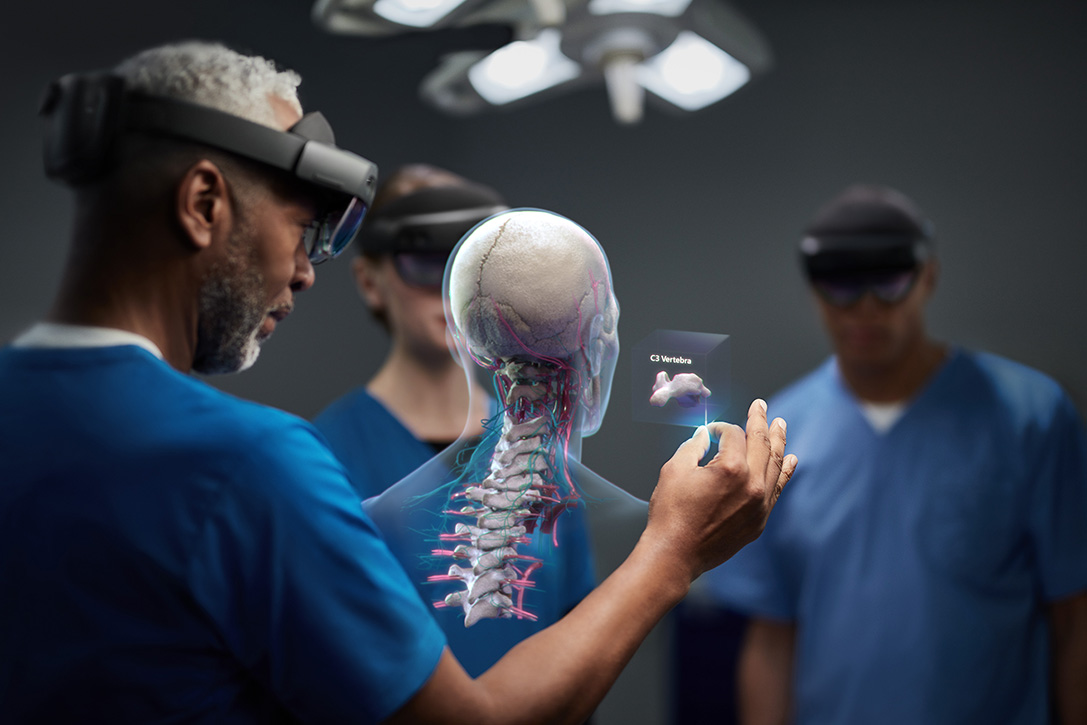
\includegraphics[width=\textwidth]{images/hologram.jpg}
    \caption{Grazie ad HoloLens l'utente può interagire con gli ologrammi}
    \label{fig:figure21}
\end{figure}

Gli ologrammi che vengono renderizzati da HoloLens appaiono nel frame olografico, direttamente davanti agli occhi dell’utente. Per effettuare il rendering HoloLens usa un display additivo, che aggiunge luce a una determinata area del frame, il che significa che è possibile vedere sia la luce emessa dal display che la luce del mondo circostante.

Gli ologrammi possono anche produrre suoni che sembrano provenire da un luogo specifico nell’ambiente. Su HoloLens, il suono proviene da due altoparlanti posizionati direttamente sopra le orecchie. Come il display olografico, gli altoparlanti sono additivi, quindi i nuovi suoni vengono introdotti senza occludere quelli provenienti dall'ambiente.

Gli ologrammi possono avere una posizione fissa all’interno dell’ambiente o seguire l’utente. Nel primo caso è anche possibile utilizzare le ancore per rendere la posizione degli ologrammi persistente anche attraverso diverse sessioni. 
Alcuni scenari invece richiedono che gli ologrammi rimangano facilmente individuabili o visibili durante la sessione. Ci sono due approcci di alto livello per questo tipo di posizionamento, chiamati \textit{display-locked} e \textit{body-locked}. 

Nel caso del display-locked i contenuti vengono fissati sul display, questo approccio crea delle complicazioni, infatti il campo visivo dell’utente viene limitato. 

Con l’approccio body-locked l’ologramma si lega al corpo dell’utente, in questo modo è possibile muoversi e spostarsi senza perderlo di vista e allo stesso tempo il campo visivo rimane inalterato.

\subsection{Mappatura Spaziale}
La mappatura spaziale genera un modello 3D dell’ambiente chiamato \textit{mesh} (Figura \ref{fig:figure22}), consentendo di posizionare oggetti virtuali su superfici reali.
Uno degli usi principali della mesh creata dalla mappatura spaziale è quello di occludere gli ologrammi, che vengono percepiti come se fossero reali. 

L'occlusione fornisce anche informazioni all'utente;
quando un ologramma viene occluso da una superficie del mondo reale, questo fornisce un feedback visivo aggiuntivo sulla sua posizione in quell’ambiente.
Inoltre, l'occlusione può anche nascondere in modo utile le informazioni all'utente; occludere ologrammi dietro i muri può ridurre il disordine visivo. 

La mappatura spaziale è utile anche nel momento in cui si vuole applicare qualsiasi tipo di forza fisica agli ologrammi, sfruttando la mesh infatti è possibile farli collidere con gli ostacoli presenti nell’ambiente.
In alcuni casi, ad esempio se sono presenti superfici in vetro o riflettenti, la mesh potrebbe essere imprecisa e non corrispondere con l’ambiente, di conseguenza le collisioni degli ologrammi potrebbero essere inaccurate. 

L'archiviazione, il rendering e l'elaborazione delle mesh possono consumare notevoli risorse di calcolo e di archiviazione.
Pertanto, ogni applicazione dovrebbe adottare uno schema di caching appropriato alle proprie esigenze, determinando quali mesh mantenere, quali scartare e quando aggiornare quelle salvate.

\begin{figure}[t]
    \centering
    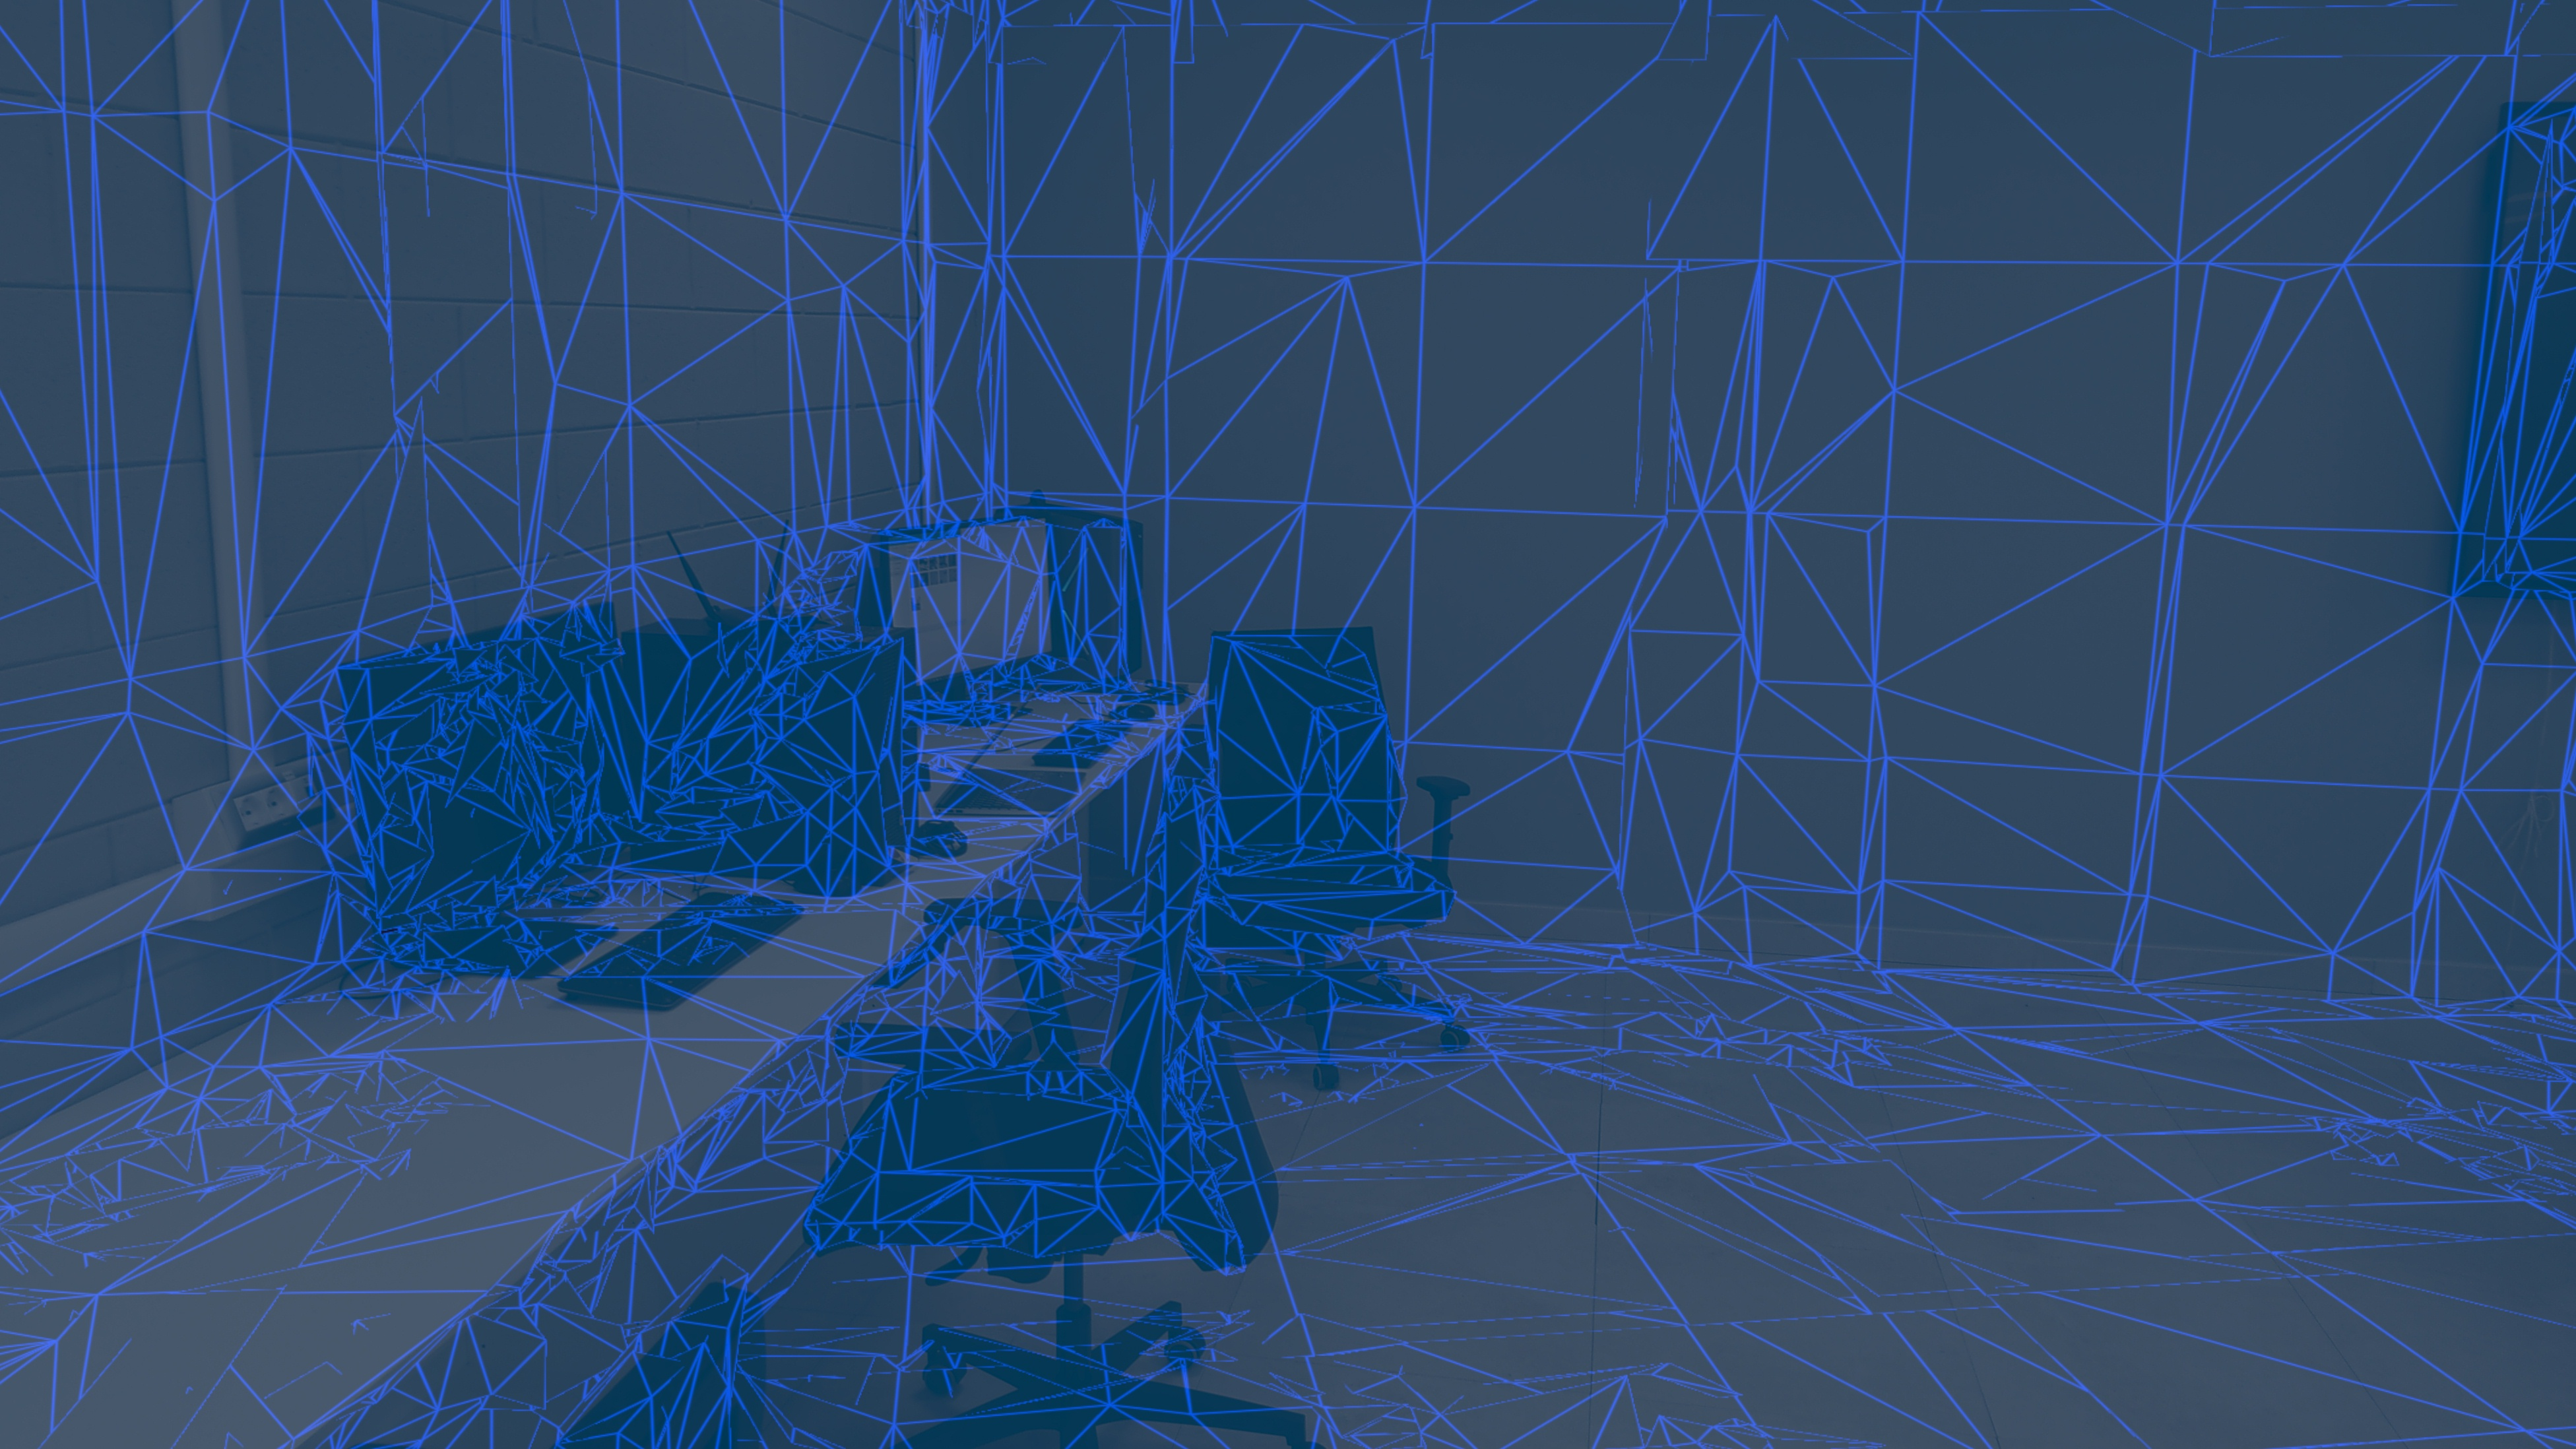
\includegraphics[width=\textwidth]{images/spatial-mapping.jpg}
    \caption{Mesh di una stanza, generata da HoloLens 2.}
    \label{fig:figure22}
\end{figure}

\subsection{Ancore}
Un’ancora rappresenta un punto nel mondo del quale il sistema tiene traccia nel tempo. Ogni ancora ha un sistema di coordinate regolabile, basato su altre ancore o sistemi di riferimento, per garantire che gli ologrammi ancorati rimangano esattamente al loro posto. È anche possibile mantenere e condividere ancore tra le sessioni dell'applicazione e tra diversi dispositivi: 

Salvando le ancore su disco e caricandole di nuovo in un secondo momento, l'applicazione può calcolare la stessa posizione nel mondo reale in più sessioni dell'applicazione su un singolo HoloLens. 

Usando i servizi Azure è possibile condividere un'ancora in cloud con più dispositivi HoloLens, iOS e Android. Facendo in modo che ogni dispositivo esegua un ologramma utilizzando la stessa ancora spaziale, gli utenti vedranno l'ologramma apparire nello stesso posto nel mondo reale. Ciò consente esperienze condivise in tempo reale. 

Le ancore condivise in cloud possono persistere anche in modo asincrono, quindi i vari dispositivi presenti nell’ambiente possono osservare e interagire con lo stesso ologramma in momenti diversi. 

Gli ologrammi che vengono ancorati purtroppo non possono essere spostati o ruotati, quindi ogni volta che si desidera interagire con un ologramma ancorato bisogna prima eliminare l’ancora, per poi crearla nuovamente nel momento in cui termina l’interazione.
Questo pone un forte limite alle esperienze condivise che sfruttano questa funzionalità;
infatti se in un ambiente sono presenti più utenti e uno di questi interagisce con un ologramma ancorato gli altri non sono in grado di vedere la fase d'interazione.

\subsection{Hand Tracking e Gaze}
La manipolazione diretta è un modello di input primario su HoloLens 2, che usa il nuovo sistema di rilevamento della mano.
HoloLens 2 è in grado di riconoscere mani e dita dell'utente (Figura \ref{fig:figure24a}) e di rilevare le collisioni con gli ologrammi, quindi è possibile interagire con questi come se fossero reali.
È anche possibile sfruttare l'indice della mano come puntatore 3D (gaze, Figura \ref{fig:figure24b}), in questo modo è possibile interagire con gli ologrammi più distanti senza doversi spostare; solitamente in un'applicazione HoloLens 2 i gaze sono due, uno per ogni mano.
Il gaze può anche essere utilizzato sfruttando gli occhi, lasciando così le mani libere.
Grazie a questa funzionalità l'utente può "fissare" l'ologramma alla testa, di conseguenza l'oggetto si muoverà e ruoterà nell'ambiente seguendo la testa dell'utente.
Le possibili interazioni con gli ologrammi sono varie, ad esempio sfruttando una mano sola si può puntare il gaze su un ologramma, unire indice e pollice (air tap) e spostare la mano nella direzione in cui si vuole posizionare l'ologramma.
Se invece si vuole ridimensionare un ologramma è necessario usare tutte e due le mani, in questo caso bisogna puntare entrambi i gaze sull'ologramma ed eseguire la gesture air tap, allargando o avvicinando le mani l'ologramma si ridimensionerà.
Un altro tipo di interazione particolarmente interessante è la rotazione dell'oggetto, per ruotare un ologramma basta eseguire la stessa procedura descritta precedentemente per il movimento, solo che invece di spostare la mano bisogna ruotarla esattamente nel modo in cui si desidera ruotare l'oggetto.

\begin{figure}[H]
    \centering
    \begin{subfigure}{0.45\textwidth}
        \centering
        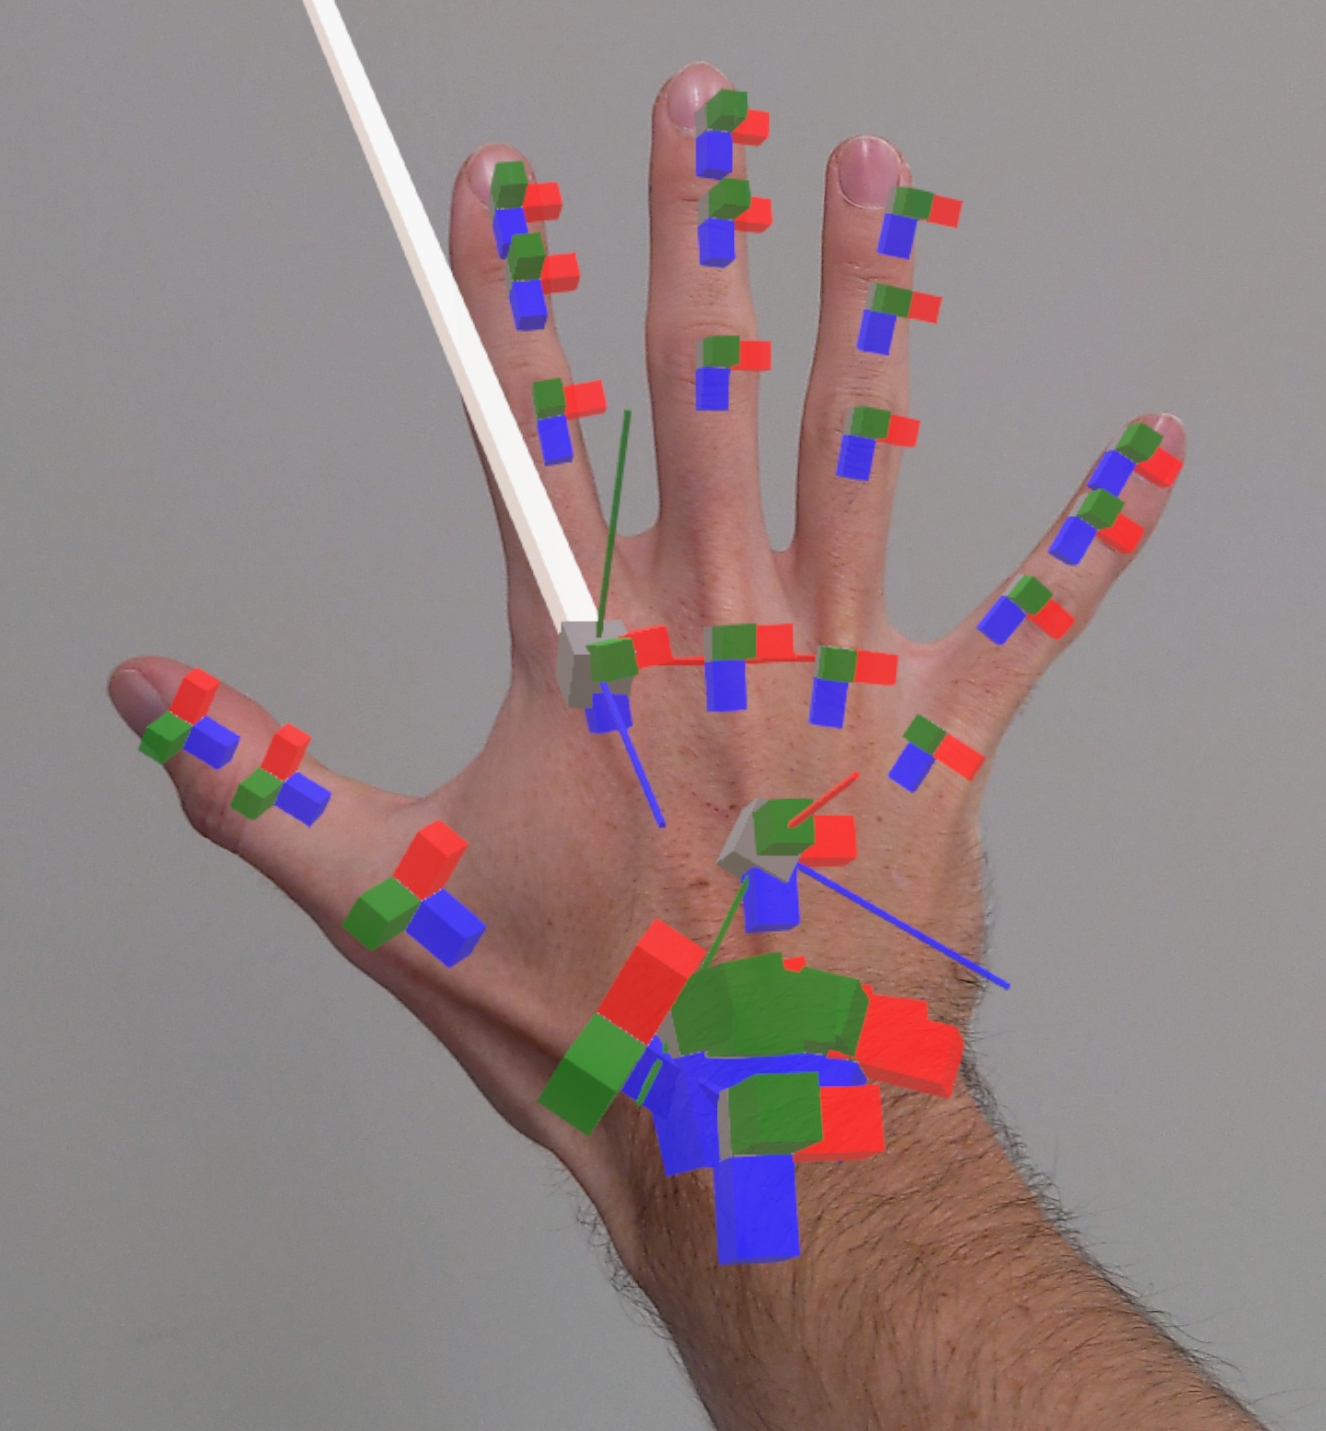
\includegraphics[width=\textwidth]{images/hand-tracking.jpg}
        \caption{Hand tracking.}
        \label{fig:figure24a}
    \end{subfigure}
    \begin{subfigure}{0.4\textwidth}
        \centering
        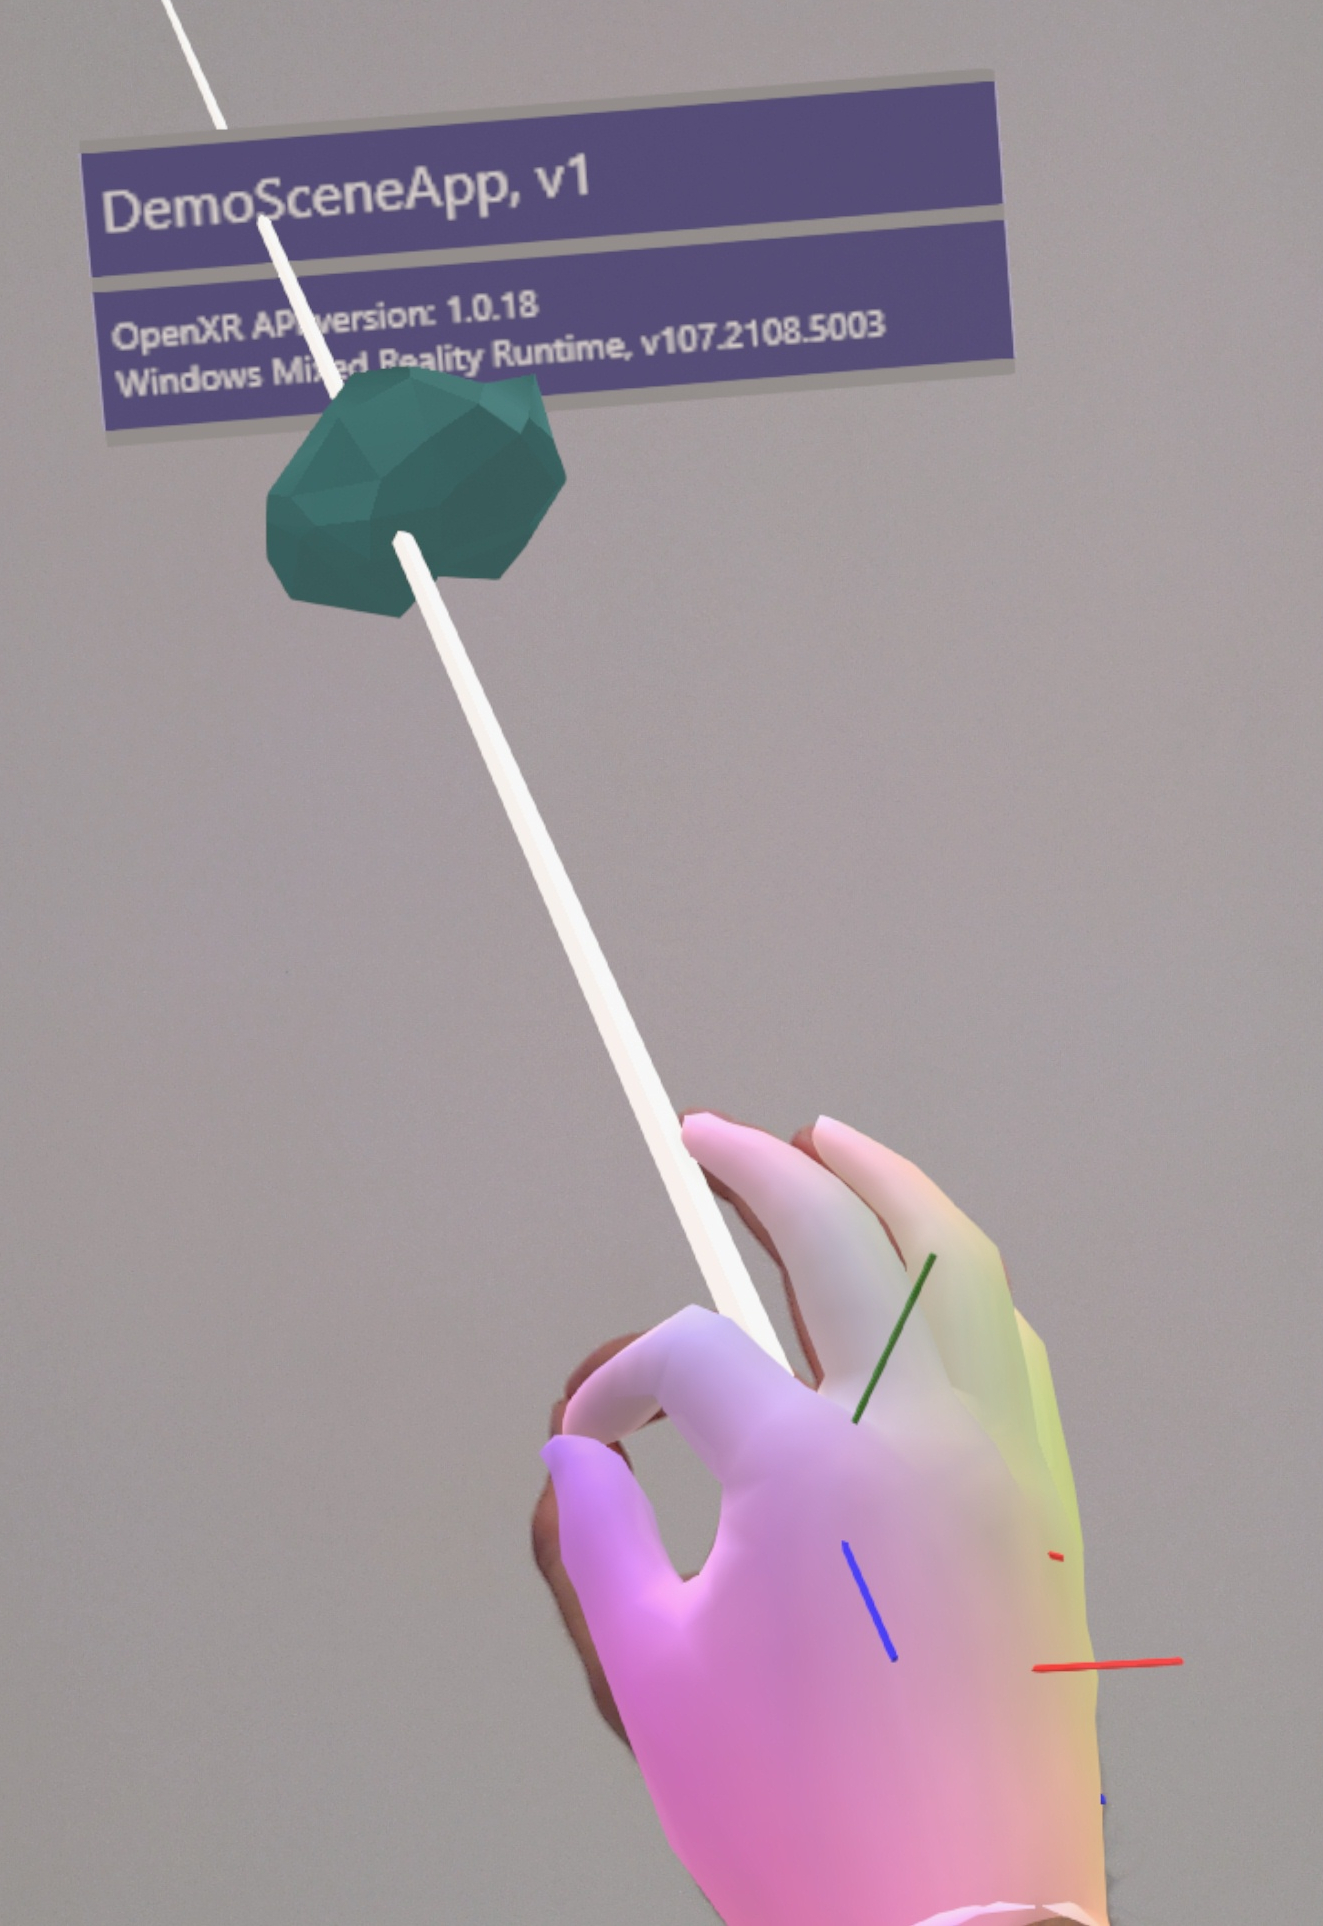
\includegraphics[width=\textwidth]{images/gaze.jpg}
        \caption{Gaze.}
        \label{fig:figure24b}
    \end{subfigure}
    \label{fig:figure24}
\end{figure}

\section{Strumenti di Sviluppo}\label{sec:Sezione2.3}
Per lo sviluppo di applicazioni HoloLens 2 esistono varie opzioni che si distinguono in base agli obiettivi e alle necessità degli sviluppatori:

\begin{itemize}
\item Unity è la piattaforma leader a livello mondiale per la creazione e l'utilizzo di contenuti 3D interattivi in tempo reale; il codice di runtime sottostante è C++, mentre lo scripting di sviluppo viene eseguito in C\#.
\item Unreal Engine 4 è un engine open source avanzato con supporto completo per la realtà mista sia in C++ che in Blueprints. 
\item Gli sviluppatori nativi che hanno esperienza nella scrittura di renderer 3D personalizzati possono creare un engine custom grazie ad OpenXR.
\item Gli sviluppatori Web che vogliono creare esperienze Web AR/VR per browser web possono usare WebXR.
\end{itemize}

Per il caso di studio si è scelto di utilizzare Unity in combinazione con il Mixed Reality Toolkit (MRTK) fornito da Microsoft, questo perché al momento è l'opzione migliore, sia dal punto di vista delle funzionalità offerte, che dalla stabilità.

MRTK per Unity è un progetto gestito da Microsoft che fornisce un set di componenti e funzionalità che consentono lo sviluppo di app di realtà mista multipiattaforma. 

MRTK è modulare, questo significa che è possibile installare in Unity solo i componenti necessari per lo sviluppo dell’applicazione; in questo modo la dimensione del progetto rimane contenuta. Inoltre, poiché è costruito con oggetti scriptabili, è anche possibile sostituire i componenti inclusi con i propri, per supportare altri servizi, sistemi e piattaforme. 

MRTK è in continuo sviluppo, vengono introdotte nuove funzionalità e risolti problemi costantemente, allo stesso tempo alcune funzionalità vengono deprecate, in base anche alle nuove versioni di Unity che vengono rilasciate. Ad oggi è possibile scegliere fra quattro opzioni, che si distinguono prevalentemente per la versione di Unity che si vuole utilizzare:

\begin{itemize}
\item L'attuale configurazione consigliata da Microsoft per HoloLens 2 e per lo sviluppo di Windows Mixed Reality è Unity 2020.3 LTS con il plug-in OpenXR più recente. 
\item Con Unity 2019 è possibile utilizzare plug-in XR integrato nell’ambiente di sviluppo. 
\item Con Unity 2021.2 il plug-in Windows XR è stato deprecato in favore di OpenXR, che quindi rimane l’unica opzione disponibile. 
\item Per Unity 2018.4 LTS è terminato il supporto di due anni e non vengono più rilasciati aggiornamenti.
\end{itemize}

I componenti del MRTK sono molti e offrono funzionalità di vario tipo: percezione ambiente, gestione dei sistemi di input e gestione delle ancore sono alcuni esempi.
La gestione di questi componenti all'interno di Unity viene affidata a dei profili specifici per ogni funzionalità.

\subsection{Sistema di Input}
Il sistema di input in MRTK consente di:
\begin{itemize}
    \item Rilevare input da una varietà di sorgenti, come controller 6DOF, mani o voce.
    \item Definire azioni astratte, come Select o Menu e associarle a diversi input.
    \item Impostare puntatori collegati ai controller per guidare i componenti dell'interfaccia utente tramite eventi del puntatore (focus e tap).
\end{itemize}

Gli input sono prodotti dagli Input Data Providers (Device Manager). Ogni provider corrisponde a una particolare fonte di input: Open VR, Windows Mixed Reality (WMR), Unity Joystick o Windows Speech, I provider vengono aggiunti al progetto tramite il profilo Registered Service Providers nel componente Mixed Reality Toolkit e producono eventi di input automaticamente quando sono disponibili le sorgenti di ingresso corrispondenti (ad esempio quando viene rilevato un controller WMR o collegato un gamepad).

Le azioni di input sono astrazioni intese a isolare la logica dell'applicazione dalle specifiche sorgenti di input. Può essere utile, ad esempio, definire un'azione Select e mapparla sul pulsante sinistro del mouse, un pulsante in un gamepad e un trigger in un controller 6DOF. È quindi possibile fare in modo che la logica dell'applicazione ascolti gli eventi dell'azione Seleziona in input invece di dover essere consapevole di tutti i diversi input che possono produrlo. Le azioni di input sono definite nel profilo delle azioni di input, che si trova all'interno del profilo Input System nel componente Mixed Reality Toolkit.

I controller vengono creati dai provider di input quando i dispositivi di input vengono rilevati e distrutti quando vengono persi o disconnessi. Il provider di input WMR, ad esempio, crea un controller WMR per dispositivi 6DOF e controller manuali WMR per le mani. Gli eventi di input generati dai controller includono l'eventuale azione di input associata.

I controller possono avere dei Pointer collegati che interrogano la scena per determinare l'oggetto di gioco con il focus e generare Pointer Event su di esso. Ad esempio, il Pointer che gestisce il gaze esegue un raycast sulla scena utilizzando la posizione del controller per calcolare l'origine e la direzione del raggio. I Pointer creati per ogni controller sono impostati nel profilo Pointer, sotto il profilo Input System.

\subsection{Percezione Ambientale}
Il sistema di percezione ambientale (Spatial Awareness) fornisce la consapevolezza ambientale del mondo reale nelle applicazioni di realtà mista. Introdotta in un'applicazione HoloLens, Spatial Awareness fornisce una mesh, che rappresenta la geometria dell'ambiente, così da consentire interazioni tra gli ologrammi e il mondo reale.
Il sistema di percezione spaziale è simile al sistema di input descritto precedentemente, in quanto i Data Provider forniscono al sistema dati su una mesh relativa al mondo reale. Il profilo Spatial Awareness deve avere almeno uno Spatial Observer registrato. Gli Spatial Observer sono generalmente componenti specifici della piattaforma che fungono da provider per fornire vari tipi di dati relativi alla mesh generata da un endpoint specifico (ad esempio HoloLens).
Il profilo Spatial Awareness permette di gestire vari aspetti per quanto riguarda la generazione della mesh, ad esempio è possibile definire la frequenza di aggiornamento (che tipicamente varia fra 0.1 e 0.5 secondi).
L'Observer può essere impostato come stazionario, ovvero viene generata solo la porzione di mesh relativa al punto dove si è avviata l'applicazione.
L'Observer ha una forma che definisce il tipo di volume della mesh che verrà utilizzato. Le opzioni supportate sono:

\begin{itemize}
    \item Cubo allineato agli assi: forma rettangolare che rimane allineata con gli assi del sistema di coordinate globali, come determinato all'avvio dell'applicazione.
    \item Cubo allineato dall'utente: forma rettangolare che ruota per allinearsi al sistema di coordinate locale dell'utente.
    \item Sfera: Un volume sferico con centro all'origine del mondo.
\end{itemize}

\subsection{Definizione dei Confini}
Il Boundary System fornisce il supporto per far visualizzare all'utente i limiti imposti dal mondo reale.
I confini definiscono l'area in cui gli utenti possono muoversi in sicurezza e sono importanti per aiutarli a evitare ostacoli mentre indossano un visore AR.

Molte piattaforme di realtà virtuale forniscono una visualizzazione automatica, ad esempio un contorno bianco sovrapposto al mondo virtuale quando l'utente o il suo controller si avvicina al confine. Il Boundary System estende questa funzionalità per consentire di visualizzare un contorno dell'area tracciata da HoloLens e fornisce altre funzionalità che possono essere utilizzate per informare agli utenti sugli ostacoli presenti nell'ambiente. 

\section{Esempio di Applicazione HoloLens 2}\label{sec:Sezione2.4}
Di seguito viene presentata un'applicazione sviluppata in PSLab durante la fase di studio della documentazione relativa ad HoloLens 2.
L'applicazione in questione è stata sviluppata con l'obiettivo di testare il sistema di gestione delle ancore, i sistemi di coordinate e le collisioni degli ologrammi con la mesh.

\subsection{Configurazione del Progetto Unity}
Esattamente come per lo sviluppo di un videogioco, è necessario inizializzare un progetto Unity.
Una volta creato il progetto è necessario importare i componenti del MRTK necessari, in modo da poter implementare le funzionalità desiderate successivamente.
Per lo sviluppo di questa applicazione sono stati utilizzati Unity 2019 e MRTK 2.5.3 ed è stato importato il componente Mixed Reality Toolkit Foundation.
A questo punto, in Unity è possibile accedere alla sezione dei profili per HoloLens 2 (Figura \ref{fig:figure25}).

\begin{figure}[t]
    \centering
    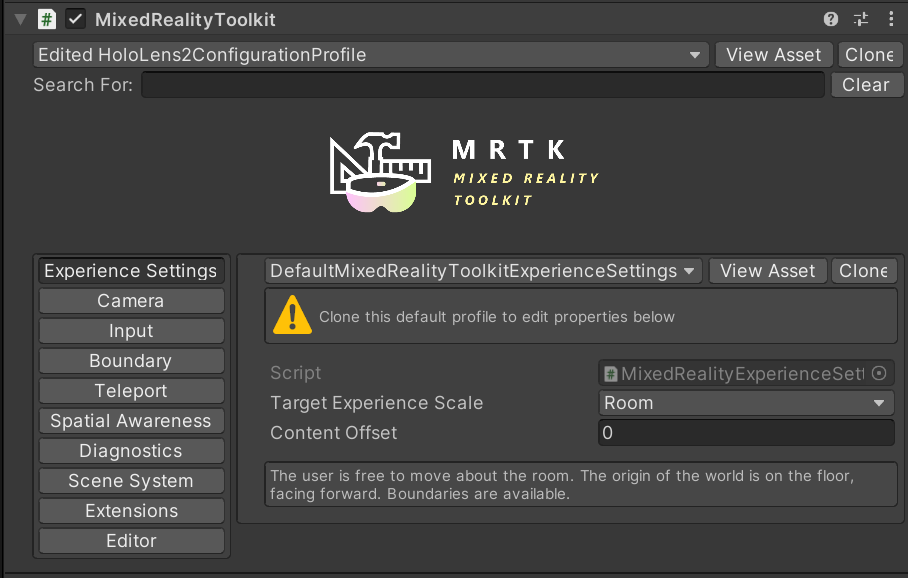
\includegraphics[width=\textwidth]{images/MRTK-profiles.png}
    \caption{Profili MRTK.}
    \label{fig:figure25}
\end{figure}

In questo caso sono state abilitate le funzionalità dei profili Spatial Awareness e Boundary System ed è stata occlusa la vista della mesh. In questo modo durante la sessione di utilizzo HoloLens 2 si occupa di mappare l'ambiente senza che l'utente se ne renda conto.

Per il posizionamento degli oggetti della scena sono stati importati in Unity il pacchetto TextMeshPro e il pacchetto \href{https://github.com/microsoft/MixedRealityLearning/releases/tag/getting-started-v2.5.0}{Tutorial Assets} di Microsoft, che offre diversi asset, utili per lo svluppo.

\subsection{Funzionamento dell'Applicazione}
Una volta importati i package correttamente è possibile aggiungere gli oggetti nella scena (Figura \ref{fig:figure26}).
In questa applicazione sono stati aggiunti:
\begin{itemize}
    \item Un cubo (\textbf{A1}) ancorato alla mesh e un modello del Rover Curiosity (\textbf{A2}) della NASA come figlio.
    \item Un cubo (\textbf{B1}) disposto su un piano (\textbf{B2}), al quale viene applicata la forza di gravità.
    \item Un cubo (\textbf{C1}) non ancorato alla mesh con una sfera (\textbf{C2}) come figlio che gli ruota attorno.
\end{itemize}

\begin{figure}[t]
    \centering
    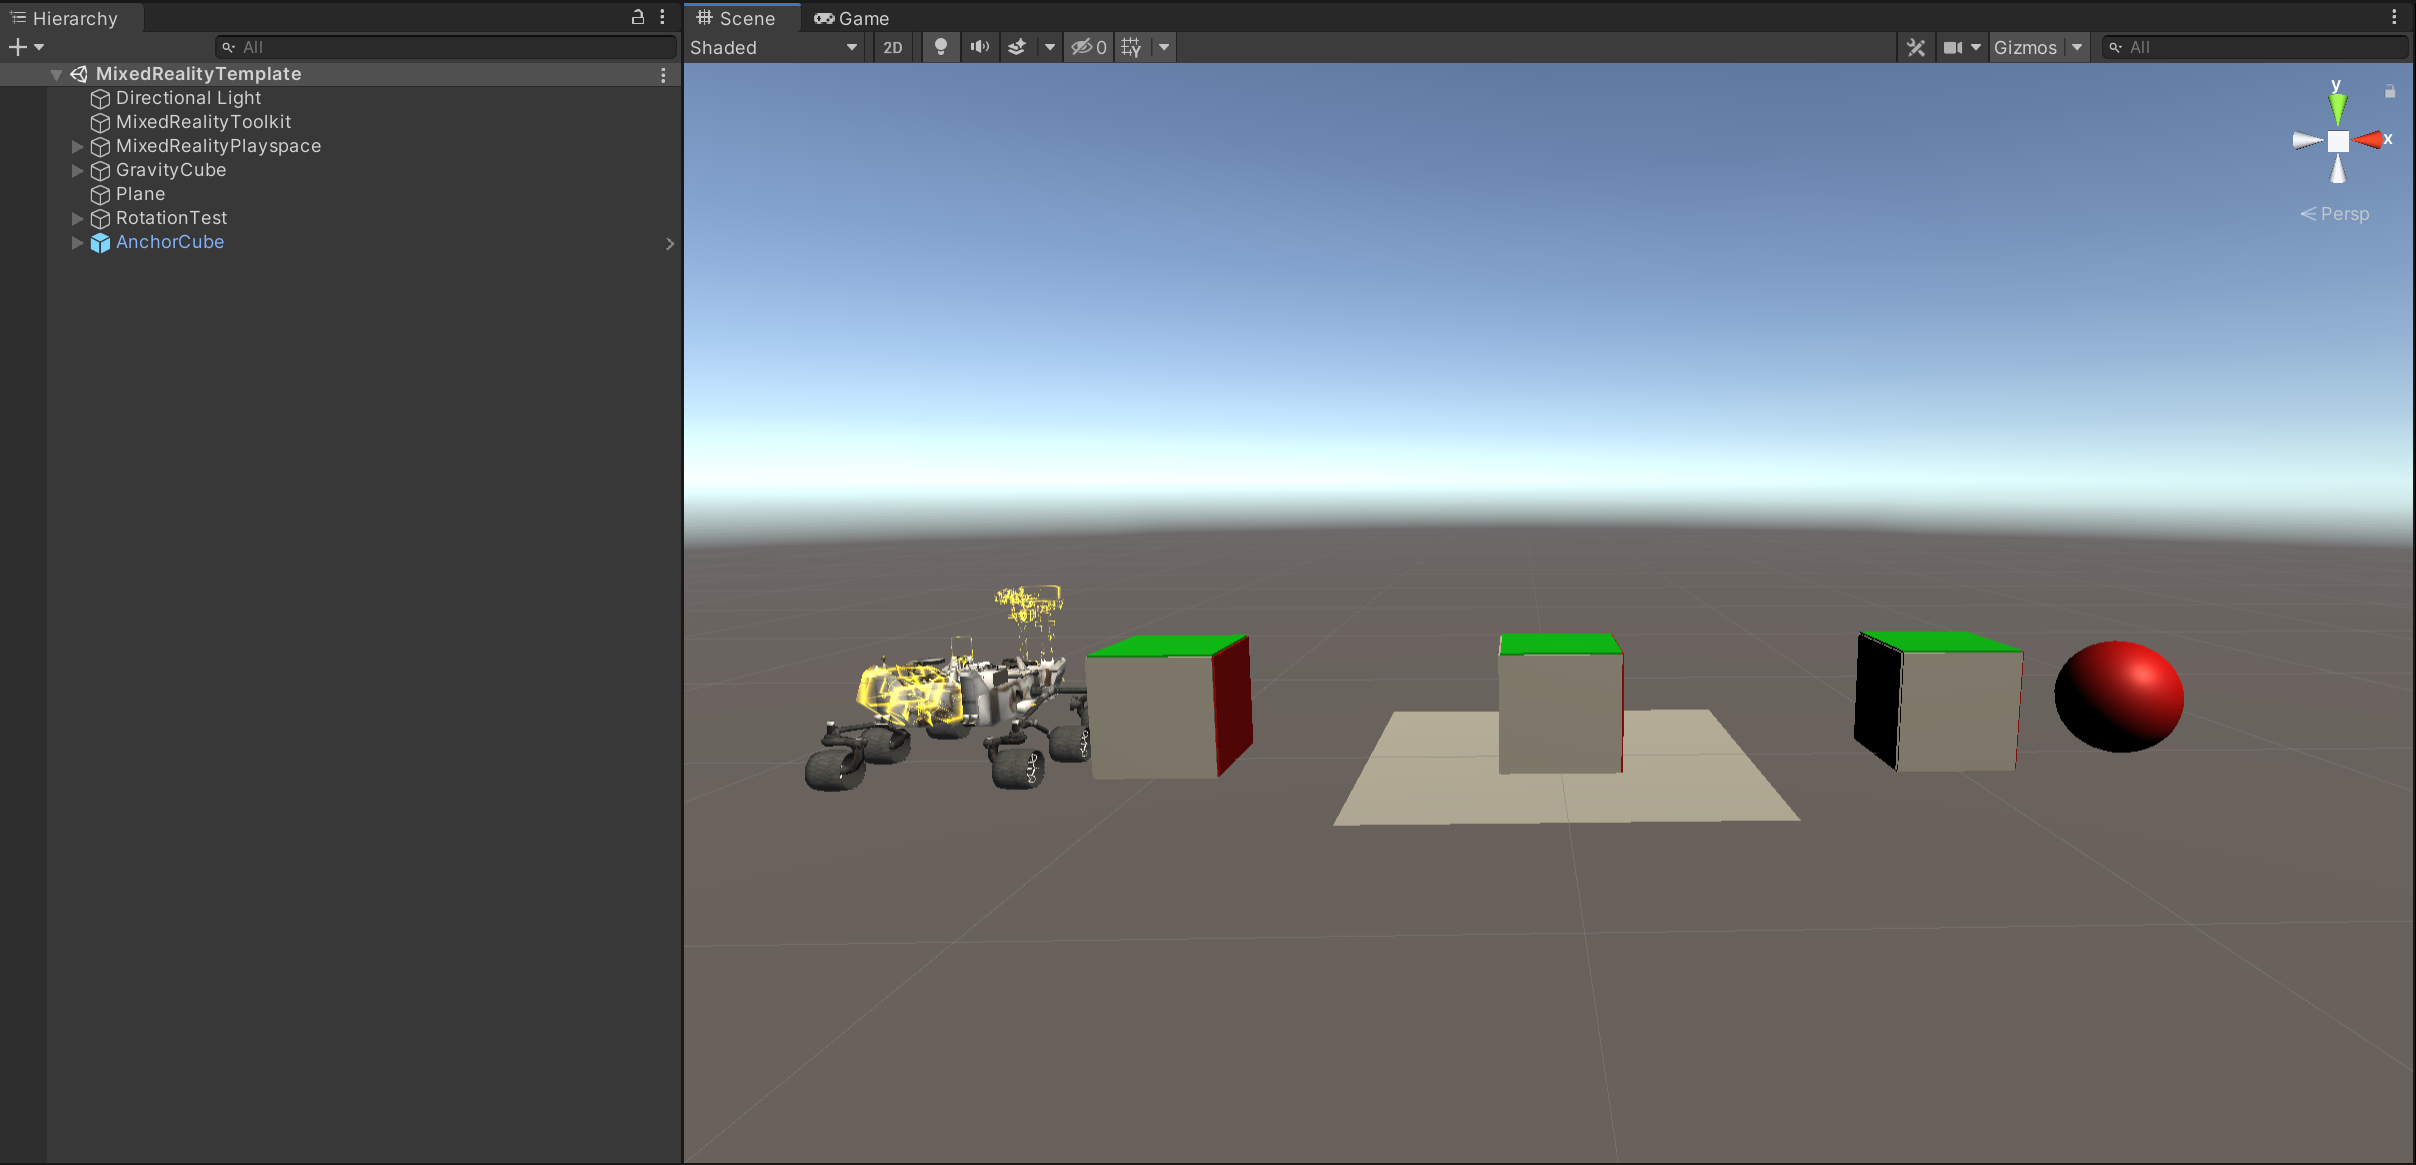
\includegraphics[width=\textwidth]{images/unity-scene.png}
    \caption{Scena di Unity.}
    \label{fig:figure26}
\end{figure}

Per abilitare la manipolazione degli ologrammi vengono aggiunti gli script Object Manipulator e NearInteractionGrabbable a tutti gli oggetti della scena, tranne che al piano \textbf{B2}. Questi due script fanno parte dei componenti del MRTK.
Object Manipulator permette di manipolare un ologramma sfruttando il gaze, così è possibile interagire con gli ologrammi anche se sono distanti. NearInteractionGrabbable abilita le interazioni da vicino, permettendo di manipolare gli ologrammi prendendoli come se fossero oggetti reali.

Sfruttando il Boundary System e il componente Spatial Mapping Collider applicato al cubo \textbf{B1} è possibile abilitare le collisioni con la mesh. Per applicare la forza di gravità è stato anche aggiunto il componente Rigid Body.
Il risultato è che nel momento in cui l'utente prende \textbf{B1}, spostandolo dal piano \textbf{B2} e lasciandolo cadere a terra, \textbf{B1} colliderà con la mesh generata da HoloLens 2, ovvero con il pavimento.
Senza la presenza della mesh \textbf{B1} oltrepasserebbe il pavimento e scomparirebbe dalla scena.

In Unity, impostando l'oggetto \textbf{C2} come figlio dell'oggetto \textbf{C1}, le coordinate di \textbf{C2} saranno stabilite sulla base di quelle di \textbf{C1}. Durante l'utilizzo dell'applicazione, spostando \textbf{C1}, \textbf{C2} si muoverà di conseguenza mantenendo la rotazione attorno a \textbf{C1}, non vale il contrario.

Per quanto riguarda la gestione delle ancore è stato sfruttato il World Anchor Store, una funzionalità del MRTK che permette di salvare la posizione di un ologramma all'interno di un ambiente (su un solo dispositivo).
È stata associata un'ancora al cubo \textbf{A1}, che viene eliminata nel momento in cui l'utente interagisce con l'ologramma e ricreata al termine dell'interazione.
L'ancora viene salvata nel World Anchor Store, che si occupa di renderla persistente e disponibile attraverso diverse sessioni.
La posizione di \textbf{A2} è comunque sempre relativa a quella di \textbf{A1}; quindi, attraverso sessioni differenti, \textbf{A1} manterrà posizione e rotazione, mentre \textbf{A2} assumerà posizione e rotazione stabilite in Unity relativamente ad \textbf{A1}. 

Per la gestione delle ancore è stato sviluppato uno script che una volta associato a un oggetto permette di salvare (listato \ref{lst:listato3}) ed eliminare (listato \ref{lst:listato2}) l'ancora associata.

\lstset{language=[Sharp]C, numbers=left}
\begin{lstlisting}[caption={Metodo richiamato per eliminare l'ancora dell'ologramma associato.}, label=lst:listato2]
    public void DeleteExistingAnchor()
    {
        WorldAnchor anchor = rootGameObject.GetComponent<WorldAnchor>();
        if (anchor != null)
        {
            Destroy(anchor);
            worldAnchorStore.Delete(rootGameObject.name);
            this.savedRoot = false;
        }
    }
\end{lstlisting}

\begin{lstlisting}[caption={Metodo richiamato per salvare l'ancora dell'ologramma associato.}, label=lst:listato3]
    public void SaveAnchor()
    {
        WorldAnchor anchor = rootGameObject.AddComponent<WorldAnchor>();
        if (!this.savedRoot && anchor != null)
        {
            this.savedRoot = this.worldAnchorStore.Save(rootGameObject.name, anchor);
        }
    }
\end{lstlisting}

Per ogni sessione, prima di utilizzare le ancore del World Anchor Store è necessario richiedere il caricamento in modo asincrono di quest'ultimo (listato \ref{lst:listato1}). Una volta caricato il World Anchor Store è possibile caricare le ancore salvate nelle sessioni precedenti (listato \ref{lst:listato4}).

\begin{lstlisting}[caption={Metodo richiamato una volta caricato il World Anchor Store.}, label=lst:listato1]
    void Start()
    {
        WorldAnchorStore.GetAsync(StoreLoaded);
    }

    private void StoreLoaded(WorldAnchorStore store)
    {
        worldAnchorStore = store;
        LoadAnchor();
    }
\end{lstlisting}

\begin{lstlisting}[caption={Metodo richiamato per reperire l'ancora dal World Anchor Store.}, label=lst:listato4]
    private void LoadAnchor()
    {
        this.savedRoot = this.worldAnchorStore.Load(rootGameObject.name, rootGameObject);
    }
\end{lstlisting}